\documentclass[12pt,a4paper]{article}

\usepackage[utf8]{inputenc}
\usepackage[T1]{fontenc}
\usepackage[top=3cm, bottom=4.5cm, left=2.8cm, right=2.8cm]{geometry}
\usepackage[pdftex]{graphicx}
\usepackage[italian]{babel}
\usepackage{bold-extra, amssymb, amsmath, mathtools, microtype, cite}
\usepackage{subcaption}
\usepackage{wrapfig}
\usepackage{relsize}
\usepackage{rotating}
\usepackage{colortbl}
\usepackage{color}
\usepackage{siunitx}
\usepackage{textcomp}
\usepackage{paracol}
\usepackage{fancyhdr}
\usepackage{svg}
\usepackage{hyperref}

\svgpath{{images/}}
\graphicspath{{images/}}

\pagestyle{fancyplain}
\headheight 35pt
\lhead{Politecnico di Torino}
%\chead{\today}
\rhead{Tecnologie per IoT}
\lfoot{}
\cfoot{}

\begin{document}

\begin{figure}[b]
\centering
\includesvg[width=0.2\textwidth]{logo_polito}
\end{figure}

%\begin{vplace}[0.15]
\title{Relazione laboratorio Software}
\author{}
\maketitle
%\begin{center}
%    \LARGE{\textbf{Relazione Laboratorio Hardware}}
%\end{center}
\vspace{10cm}
\begin{center}Davide Miola\\Elia Fontana\end{center}
%\end{vplace}

\newpage
\setcounter{page}{1}
\rfoot{\thepage}
%\thispagestyle{myheadings}
\section{Prima Parte}

Il primo laboratorio si concentra, con l'eccezione dell'ultimo esercizio, attorno allo stesso concetto: conversioni di valori di temperatura tra le più comuni unità di misura.
Per questo, è sembrato conveniente dedicare del tempo a organizzare il codice volto ad eseguire le conversioni in un unico file sorgente, che viene quindi condiviso tra i vari esercizi: questo è il file \verb|SW/part1/conversions.py|
\\ \\
La strategia adottata per gestire conversioni tra una qualsiasi coppia di unità supportate prevede di passare in ogni caso attraverso i Kelvin, in modo da ridurre la quantità di codice necessario.

In particolare, il file \verb|conversions.py| contiene le funzioni in grado di effettuare la conversione da una qualsiasi unità a Kelvin e viceversa; queste funzioni non sono tuttavia pensate per essere usate direttamente dall'esterno, piuttosto sono sfruttate dalla funzione \verb|convert(...)|, la quale accetta un valore in input con la sua unità, nonché l'unità target, e restituisce il valore convertito (nel caso di temperature fisicamente impossibili - cioè se il suo valore in Kelvin risulta negativo - viene sollevata un'eccezione di tipo \verb|ValueError|).

\noindent In aggiunta a \verb|convert(...)|, è disponibile nello stesso file anche \verb|convertMultiple(...)|, che si occupa di eseguire la conversione di una lista di valori.
\\ \\
A questo punto, l'implementazione dei singoli esercizi si è rivelata molto semplice, e le uniche note che mi piacerebbe sottolineare riguardano alcune funzionalità comuni di \textit{Quality of Life}, tra cui una modalità per permettere di terminare l'esecuzione di programmi basati su CherryPy che verrà adottata per ogni esercizio in cui è applicabile, e che consiste semplicemente nel rispondere a richieste \verb|GET| a \verb|/shutdown| con la terminazione dello script; inoltre il gruppo si è discostato dalle indicazioni sulle slide del corso per quanto riguarda l'impostazione di codici di errore HTTP tramite CherryPy: piuttosto che generare l'apposita eccezione, viene semplicemente modificato il codice di stato nel messaggio di risposta con \verb|cherrypy.response.status = ...|, in modo da poter avere piena libertà sull'effettivo messaggio di risposta pur mantenendo il corretto codice di errore.

\begin{figure}[h]
    \centering
    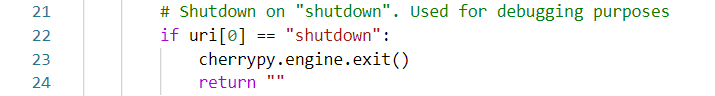
\includegraphics[width=0.9\textwidth]{shutdown.png}
    \caption*{\texttt{SW/part1/es01.py}: Metodologia adottata per la terminazione dei programmi basati su CherryPy.}
    \label{fig:shutdown}
\end{figure}

Per quanto riguarda l'esercizio quattro, è stato sufficiente abilitare il supporto di CherryPy al servizio di contenuto statico, in particolare linkando la directory contenente gli asset di Freeboard (\verb|./freeboard|) con la root del servizio web (\verb|/|), nonché esplicitando il file \verb|index.html| da utilizzare così da vedersi servita la homepage di freeboard a \verb|http://host:port/|. Dopodiché, abbiamo implementato il metodo \verb|POST| in modo che ricevesse la configurazione di Freeboard in formato JSON e la salvasse nel file \verb|freeboard/dashboard/dashboard.json| come richiesto dalle specifiche.

\begin{figure}[h]
    \centering
    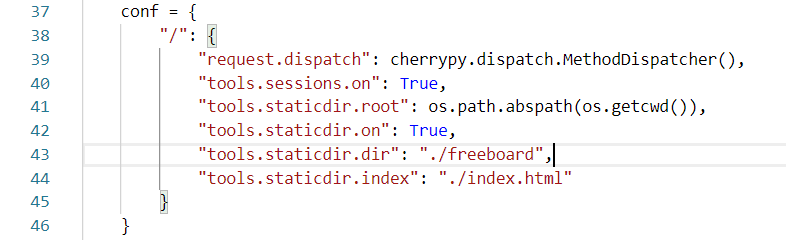
\includegraphics[width=0.9\textwidth]{static.png}
    \caption*{\texttt{SW/part1/es04.py}: Dizionario di configurazione di CherryPy per abilitare il contenuto statico.}
    \label{fig:static}
\end{figure}

\section{Seconda Parte}

\subsection{Catalog}

L'esercizio più significativo del secondo laboratorio software è sicuramente il numero uno, e il cinque dopo di lui. Viene, in questi esercizi, introdotto il concetto di \textit{Service/Device Catalog}, che verrà utilizzato non solo dagli altri esercizi dello stesso laboratorio, ma anche da tutti i successivi esercizi, anche di altri laboratori.
\\ \\
Nella nostra implementazione, il catalogo è rappresentato dalla classe \verb|RESTCatalog|, che innanzitutto implementa, tra i vari metodi REST messi a disposizione da CherryPy, \verb|GET| e \verb|PUT|.

La classe principale, poi, viene \textit{estesa} in funzionalità tramite \textit{moduli}, definiti come sottoclassi di \verb|RESTCatalog|: tra questi \verb|TimeoutManagerRunner| è presente già nella prima versione (esercizio uno), mentre \verb|MQTTDeviceSubscriptionListener| viene aggiunto dal quinto esercizio.
\\ \\
\begin{figure}[htbp]
    \centering
    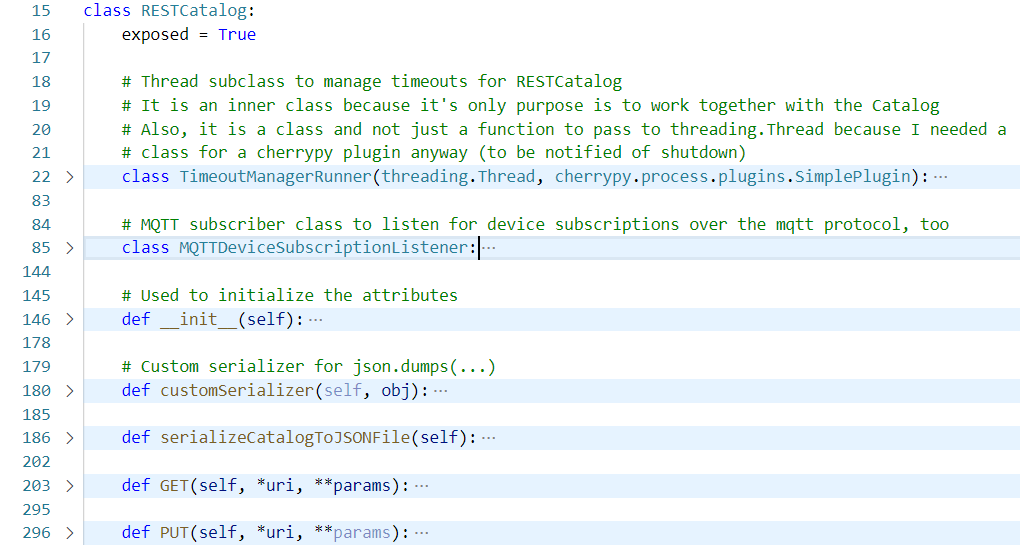
\includegraphics[width=0.9\textwidth]{catalog.png}
    \caption*{\texttt{SW/part2/es05.py}: Struttura di base ad alto livello del catalogo.}
    \label{fig:catalog}
\end{figure}
Il funzionamento di base prevede che \verb|RESTCatalog| includa l'intero database di utenti, dispositivi, nonché servizi correntemente iscritti al catalogo, all'interno di un dizionario Python. Tale struttura dati è organizzata nel seguente modo:
\begin{verbatim}
                  {
                      "devices": {<deviceID>: d, ...},
                      "services": {<serviceID>: s, ...},
                      "users": {<userID>: u, ...}
                  }
\end{verbatim}

Ogni entità (vale a dire ogni dispositivo, servizio o utente), viene memorizzato non attraverso il JSON che lo descrive, bensì come istanza della classe corrispondente. Abbiamo infatti deciso di implementare le classi \verb|Device|, \verb|Service|, \verb|User|, nonchè \verb|EndPoint|, puramente per eleganza del codice, e per preservarne la scalabilità futura.

Di fatto, l'aggiunta di una qualsiasi nuova entità al database del catalogo procede secondo la seguente modalità:
\begin{enumerate}
    \item L'utente esegue la richiesta \verb|PUT| al catalogo fornendo il JSON che descrive l'entità che si vuole iscrivere;
    \item Viene controllata la validità del JSON ricevuto, dopodiché si usa il metodo statico messo a disposizione dalla classe target (i.e. \verb|Device|, \verb|Service| o \verb|User|) per eseguire il \textit{parse} dell'oggetto, quindi restituirne l'istanza corrispondente;
    \begin{figure}[htbp]
    \centering
    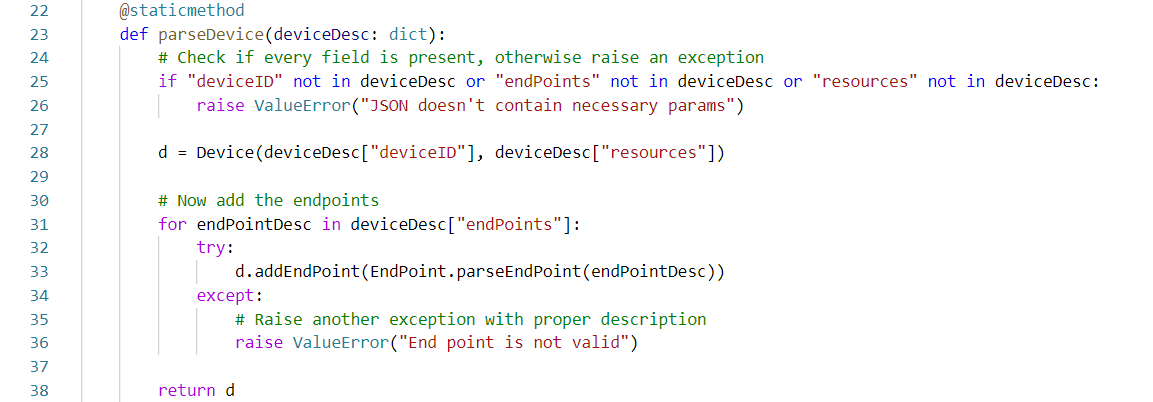
\includegraphics[width=0.95\textwidth]{parse_device.png}
    \caption*{\texttt{SW/part2/Device.py}: Funzione di \textit{parse} dell'entità \textit{Device}.}
    \label{fig:parse_device}
\end{figure}
    \item Il catalogo a questo punto aggiunge il timestamp all'oggetto ricevuto;
    \item L'oggetto viene aggiunto al database;
    \item Si scatena la sincronizzazione delle modifiche al database con la sua versione in memoria secondaria.
\end{enumerate}

Il catalogo, infatti, mantiene una copia persistente del database in un file locale, chiamato \textit{catalog.json}; per poter serializzare il database in un unico documento JSON, abbiamo scritto, per ogni oggetto, un metodo \verb|serialize()|, il quale è richiamato dal nostro \textit{custom serializer}, che viene quindi passato a \verb|json.dumps(...)|.

\begin{figure}[htbp]
    \centering
    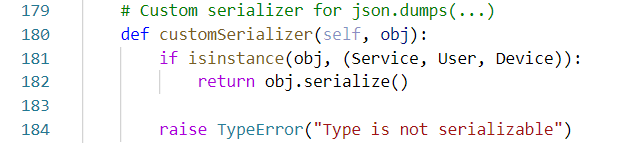
\includegraphics[width=0.75\textwidth]{custom_serializer.png}
    \caption*{\texttt{SW/part2/es05.py}: Funzione \texttt{customSerializer(...)}.}
    \label{fig:custom_serializer}
\end{figure}

Della gestione della rimozione automatica delle entità con un timestamp di iscrizione troppo vecchio se ne occupa il modulo \verb|TimeoutManagerRunner|: la classe estende \verb|threading.Thread|, in modo che il suo metodo \verb|run()| possa essere eseguito in un thread indipendente da quello principale; implementa inoltre \verb|cherrypy.process.plugins.Sim-| \verb|plePlugin|. Così, la classe si configura come plugin di CherryPy, il che ci permette di essere notificati della terminazione del servizio web per poter terminare anche i thread aggiuntivi (è l'unica funzionalità offerta da CherryPy di cui ci avvaliamo).

Il modulo, sostanzialmente, esegue in modo periodico la scansione di tutte le entità presenti nel database del catalogo (a cui quindi deve avere accesso), ed elimina quelli che ritiene essere troppo vecchi, quindi chiama \verb|catalog.serializeCatalogToJSONFile()| per sincronizzare le modifiche con il file \textit{catalog.json}.
\\ \\
Infine, il modulo \verb|MQTTDeviceSubscriptionListener| si occupa di accettare messaggi MQTT al topic \verb|/tiot/19/catalog/addDevice|, al quale si iscrive; nel metodo \verb|onMessage(...)|, quindi, deserializza il JSON ricevuto ed aggiunge il nuovo dispositivo (se valido) al database globale.

\subsection{Restanti esercizi}

Gli esercizi rimanenti, a questo punto, risultano piuttosto immediati, e si riducono, nella maggior parte dei casi, a semplici server HTTP.
\\ \\
L'esercizio due presenta un semplice menu testuale, che permette di selezionare tutte le separate funzionalità, implementate con la libreria \verb|requests|.
\\ \\
Degli esercizi immediatamente successivi, l'unica cosa degna di essere sottolineata riteniamo essere la metodologia per gestire le periodiche sottoscrizioni al catalogo: in entrambi i casi viene impiegato una sottoclasse che estende \verb|threading.Thread| in modo da poter ripetere la sottoscrizione in modo periodico.
\\ \\
Infine, l'ultimo esercizio utilizza \verb|paho.mqtt| per emulare il dispositivo IoT.

\section{Terza Parte}

\subsection{Esercizi Due e Tre}

Lo sketch Arduino utilizzato per pubblicare le letture di temperatura è molto simile agli ultimi esercizi del laboratorio hardware; la differenza più significativa è probabilmente il codice che si occupa di effettuare la sottoscrizione periodica al Device Catalog.

Data l'ultima versione del Catalog sviluppata nell'esercizio cinque del precedente laboratorio software, dovevamo scegliere tra l'iscrizione tramite richiesta \verb|PUT| HTTP, oppure tramite pubblicazione sul topic MQTT apposito. Alla fine si è optato per la seconda possibilità, puramente per via della maggiore semplicità implementativa in codice Arduino.

Lo sketch, semplicemente, definisce la stringa di descrizione della Yùn usata per la sottoscrizione in memoria flash (usando la macro \verb|F(...)|), e la pubblica con periodo di \SI{60}{\second} sul topic \verb|/tiot/19/catalog/addDevice|.
\\ \\
Dal punto di vista del server Python, la prima operazione da effettuare è ovviamente la richiesta al Catalog del \textit{device descriptor} associato alla Yùn. Questo avviene con una semplice richiesta \verb|GET| a \verb|/getDevice?id=Yun|, dove \verb|Yun| è il codice del dispositivo ricercato (il cui valore è \textit{hardcoded} nel sorgente del server). Dopodiché, viene scorsa la lista di \textit{resources} esposte dal dispositivo alla ricerca di quella etichettata con \textit{temperature} (o \textit{led}), il cui indice viene usato per risalire allo specifico end point MQTT usato dall'Arduino per pubblicare i valori di temperatura (o su cui ascolta per lo stato del led).
\\ \\
Tutto questo è reso possibile da un'implicita specifica formale che ci siamo sforzati di applicare ad ogni esercizio, che consiste nel mantenere una corrispondenza biunivoca tra la lista di risorse di un dispositivo e la corrispondente lista di end point; questo sta a significare che, per esempio, se la terza risorsa (nell'ordine specificato dal dispositivo stesso) è la temperatura, ci aspettiamo che l'end point a cui tale risorsa sia resa disponibile debba essere la terza nella lista di end point.
\\ \\
Una piccola differenza rispetto alle implementazioni precedenti può essere osservata nella gestione del thread aggiuntivo che si occupa di mantenere aggiornata la sottoscrizione dei servizi web al Service Catalog: piuttosto che creare un'intera classe che estenda \verb|threading.Thread|, si è qui optato per la definizione di un oggetto di tipo \verb|threading.Thread| tramite il costruttore che ne accetta la funzione \verb|run()| attraverso il parametro \verb|target|.
\\ \\
In entrambi i casi, infine, la chiusura del programma avviene quando l'utente preme il tasto `\verb|q|'.

\subsection{Esercizio Quattro}

In questo ultimo esercizio guidato viene ripreso lo \textit{smart home controller} basato su Arduino che era stato costruito durante i laboratori hardware, e viene adeguato al concetto di IoT: il nodo sensore (nel nostro caso la Yùn), si limita a raccogliere i rilevamenti dei vari sensori di cui è equipaggiato per trasmetterli tramite Internet ad un server remoto (implementato in Python), il quale si deve occupare quindi di processare questi dati per poi ritrasmettere all'Arduino i comandi di attuazione adeguati.
\\ \\
Sulla carta, tutto questo è molto semplice ed elegante, tuttavia, durante l'implementazione, il nostro gruppo si ritrovato a dover affrontare non pochi problemi, legati soprattutto alla natura \textit{embedded} della Yùn. Andiamo per ordine.
\\ \\
Lo sketch Arduino deve:
\begin{itemize}
    \item Leggere i valori riportati dai sensori;
    \item Pubblicarli tramite MQTT;
    \item Rimanere in ascolto di messaggi MQTT contenenti comandi di attuazione relativi al led, al motore DC, e al display;
    \item Iscriversi periodicamente al device catalog.
\end{itemize}

Purtroppo, sembra che, rispetto alla versione completamente locale della stessa applicazione, la Yùn abbia molto più lavoro da sbrigare; ma il problema più grande, nonostante tutto, non si è rivelato essere la limitata velocità di elaborazione del suo microcontrollore da appena \SI{16}{\mega\hertz}, bensì la ancora più esigua quantità di memoria installata a bordo della scheda. A sketch completato, infatti, erano comuni problemi simili a quelli descritti alla fine della relazione del laboratorio hardware, cioè l'invio di messaggi MQTT vuoti, errori inspiegabili durante la deserializzazione di documenti JSON, eccetera.
\\ \\
Alla fine, il problema fu circoscritto al codice responsabile della sottoscrizione periodica della board al catalogo, il quale infatti si affidava ad una lunga stringa contenente il JSON di descrizione della Yùn. Non era semplicemente disponibile sufficiente memoria contigua per gestire una stringa di circa 400 caratteri.

Per questo, dopo esserci consultati con il professor Pagliari, si è deciso di sollevare il microcontrollore AVR di questo onere, e piuttosto utilizzare uno \textit{script sh} memorizzato nella memoria permanente del sottosistema Linux della Yùn per effettuare le iscrizioni al catalogo, così che dallo sketch Arduino si sarebbe dovuto semplicemente richiamare tale script.

\begin{figure}[htbp]
    \centering
    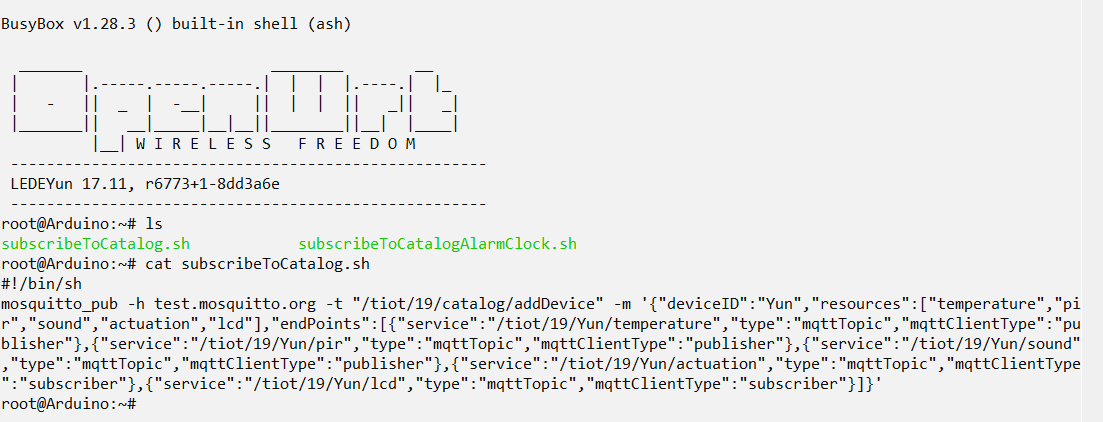
\includegraphics[width=0.85\textwidth]{sh.png}
    \caption*{\texttt{SW/part3/es04/subscribeToCatalog.sh}: Lo script usato per effettuare la sottoscrizione al Device Catalog.}
    \label{fig:sh}
\end{figure}

In questo modo, siamo riusciti a contenere l'utilizzo di memoria, e ottenere quindi un comportamento deterministico da parte della Yùn.
\\ \\
Per quanto riguarda il server remoto, il suo funzionamento è costruito attorno ad un loop principale (\verb|mainLoop()|) attestato su un thread secondario in modo che possa essere eseguito periodicamente: date le informazioni raccolte tramite MQTT (da topic ricavati in maniera simile a quanto fatto negli esercizi precedenti), \verb|mainLoop()| si occupa di decidere se le rilevazioni sono in accordo con la presenza o meno di una persona, regolare i set point di conseguenza, nonché inviare i comandi di attuazione e/o aggiornare il contenuto visualizzato sul display connesso alla Yùn (il tutto utilizzando esclusivamente SenML per ogni comunicazione).

Il meccanismo che permette di modificare i set point consiste semplicemente nel effettuare una richiesta \verb|POST| al servizio web secondo la sintassi documentata nel codice.

Il resto rimane, tutto sommato, abbastanza standard, ed in linea con quanto già commentato per gli esercizi precedenti.
\\ \\
Arrivando quindi alle conclusioni, non possiamo che apprezzare l'indiscutibilmente maggiore flessibilità che una soluzione completamente basata sull'Internet - come quella appena descritta - assicuri rispetto ad un approccio completamente locale alla Yùn, tuttavia siamo contemporaneamente preoccupati riguardo alla scalabilità offerta da una tale soluzione, che vede il nodo sensore, nella nostra implementazione, praticamente al limite di quello che può offrire.

Per questo, diventa interessante un'ipotetica via di mezzo tra quanto sopra delineato e ciò che era stato implementato durante i laboratori hardware, ossia qualcosa in cui l'Arduino possa mantenere una maggiore autorità, pur continuando a scambiare messaggi di sincronizzazione e aggiornamento con il cloud.

\begin{figure}[htbp]
    \centering
    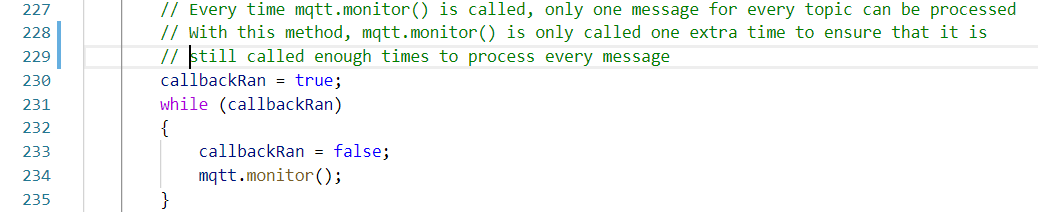
\includegraphics[width=0.9\textwidth]{mqtt_monitor.png}
    \caption*{\texttt{SW/part3/es04/es04.ino}: \texttt{callbackRan} viene settato in ogni funzione di callback per ogni topic. In questo modo riusciamo a processare tutti i messaggi ricevuti dalla precedente iterazione di \texttt{loop()}.}
    \label{fig:mqtt_monitor}
\end{figure}

\section{Quarta Parte}

\subsection{Orologio-Sveglia}

Il progetto è molto semplice, e richiama per molti aspetti il funzionamento dello \textit{Smart Home Controller} in versione remota. L'idea è quella di convertire la Yùn in un orologio-sveglia connesso ad Internet, in modo che permetta la customizzazione delle sveglie nel modo più flessibile possibile.
\\ \\
L'Arduino visualizza sul display I\textsuperscript{2}C, in ogni istante, l'orario attuale nel formato HH:mm:ss, utilizzando il led rosso per scandire i secondi, come farebbe ogni orologio digitale; mantiene, inoltre, l'iscrizione al Device Catalog allo stesso modo di come succedeva nel precedente esercizio.
\\ \\
Il server Python, intanto, instaura un'interfaccia HTTP attraverso la quale gli utenti possono aggiungere nuove sveglie tramite richieste \verb|POST|, specificando l'orario, oppure possono eliminare tutte le sveglie tramite il metodo HTTP \verb|DELETE|.

Il server remoto, tuttavia, non si limita a tenere traccia delle sveglie impostate dagli utenti, ma ha anche il compito di mantenere sincronizzato l'orologio della board Arduino inviando frequenti messaggi di sincronizzazione tramite MQTT.
\\ \\
Quando una sveglia deve essere attivata, il server invia un particolare messaggio al nodo sensore che funge da \textit{trigger} per scatenare la sveglia; poiché il messaggio non deve trasportare nessuna informazione se non la notifica di attivazione della sveglia, non viene usato il formato SenML, piuttosto viene semplicemente inviato un `\textit{1}'.
\\ \\
Al ricevimento del segnale di attivazione, l'Arduino attiva la ventola a massima velocità (nella nostra dotazione è la componente che maggiormente si avvicina ad uno speaker); a questo punto, l'utente che vuole disattivare la sveglia dovrà battere le mani due volte.

Poiché, inoltre, ci rendiamo conto che l'intensa luce blu emanata dal display connesso all'Arduino potrebbe risultare fastidioso durante la notte, abbiamo implementato una funzione per cui la retroilluminazione viene attivata solamente quando l'utente scorre la mano davanti alla sveglia (utilizzando il sensore pir), e rimane attiva, successivamente, solo per qualche secondo.

\subsection{Bot Telegram}

Il secondo progetto era decisamente più ambizioso di quello della sveglia. Il bot si propone, a tutti gli effetti, come un'interfaccia verso l'esterno dell'intero catalogo. Avviando una comunicazione con il bot si ottiene l'intera lista di tutti i dispositivi e i servizi attualmente connessi al catalogo. A questo punto l'utente può selezionarne uno per ricevere informazioni, consultare gli end point che tale entità mette a disposizione, nonché ottenere un grafico per le risorse che lo supportano.
\\ \\
L'intero programma è realizzato in Python; per il bot ci siamo affidati alla libreria \textit{python-telegram-bot}, che fornisce, oltre all'API base di Telegram, anche una API di più alto livello che si propone di risparmiare del tempo allo sviluppatore (\textit{telegram.ext}).

Per creare e configurare il bot, Telegram mette a disposizione un ulteriore bot, chiamato \textit{BotFather}, il quale fornisce il \textit{token} che permette di sviluppare il bot stesso (il \textit{token} funge contemporaneamente da login e password, è quindi una stringa che, da sola, determina il possesso di un bot).

Il \textit{token} viene quindi passato a \textit{python-telegram-bot} per inizializzare la libreria, dopodiché si devono aggiungere gli \textit{handler}, che hanno il compito di gestire varie forme di input da parte dell'utente, come l'inserimento di un comando (preceduto da `\textit{/}'), invio di testo, oppure la pressione di un bottone.

In particolare, il bot configura il comando \textit{start}. Questo comando è speciale, in quanto viene inviato automaticamente quando viene per la prima volta iniziata una nuova conversazione con il bot. Il nostro bot risponde quindi a \textit{start} con un messaggio di benvenuto, quindi viene richiamato il menu principale.

\begin{figure}[htbp]
    \centering
    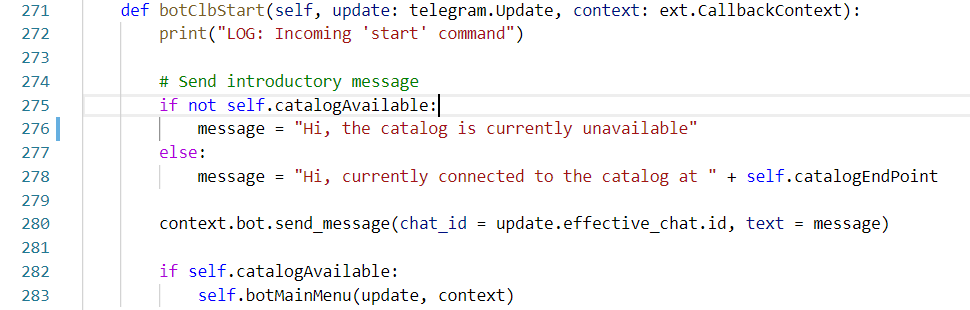
\includegraphics[width=0.9\textwidth]{bot_clb_start.png}
    \caption*{\texttt{SW/part4/telegramBot/main.py}: Il callback dell'handler del comando \texttt{/start}.}
    \label{fig:bot_clb_start}
\end{figure}

\noindent Il menu principale, così ci piace chiamarlo, non è altro che una serie di messaggi che il bot invia all'utente contenenti tutte le informazioni disponibili sul catalogo. In particolare, vengono presentate all'interlocutore la lista di dispositivi e quella di servizi correntemente disponibili presso il catalogo.
\newpage
\begin{figure}
    \centering
    \begin{subfigure}[b]{0.49\textwidth}
        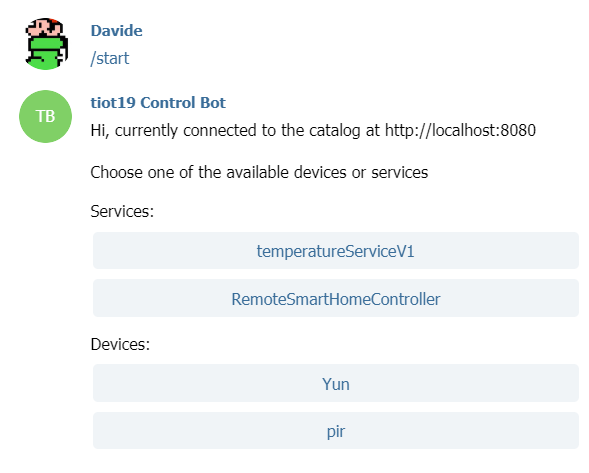
\includegraphics[width=\textwidth]{bot_main_menu.png}
        \caption{Menu principale del bot.}
        \label{fig:bot_main_menu}
    \end{subfigure}
    \begin{subfigure}[b]{0.49\textwidth}
        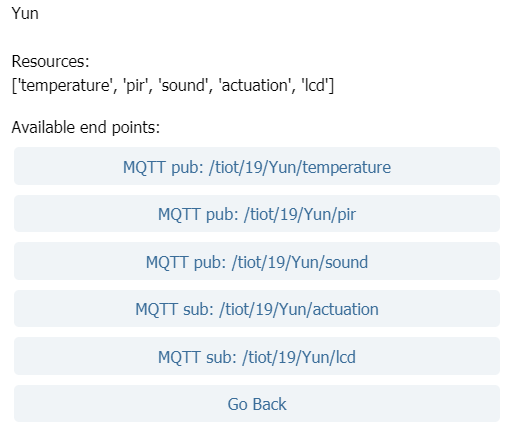
\includegraphics[width=\textwidth]{bot_yun_submenu.png}
        \caption{Sottomenu dedicato al dispositivo `\textit{Yun}'.}
        \label{fig:bot_yun_submenu}
    \end{subfigure}
\end{figure}

\noindent Ognuna di queste entità è rappresentata in chat come un bottone che l'utente può premere; il server quindi intercetta il comando con un \textit{CallbackQueryHandler}, al quale è passata la stringa che è stata specificata durante la definizione del bottone, in modo che la richiesta dell'utente possa essere identificata.

A questo punto, il bot presenta all'utente le informazioni che corredano l'entità selezionata, accompagnate da tanti ulteriori bottoni quanti sono gli end point di tale entità.
\\ \\
L'idea è quella di abilitare il server che fornisce il bot di Telegram ad interagire con ogni tipo di end point; nel caso del tipo \textit{MQTT/publisher}, viene fornito all'utente un grafico delle ultime 64 rilevazioni.

\begin{figure}[htbp]
    \centering
    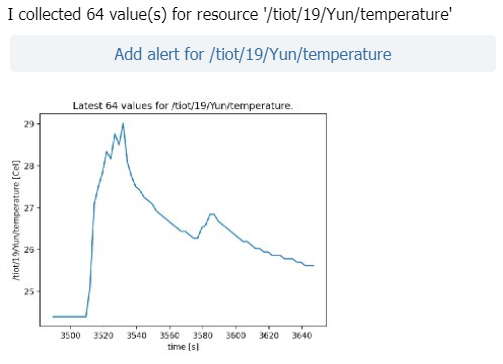
\includegraphics[width=0.65\textwidth]{bot_temp_graph.png}
    \caption*{Esempio di di grafico per la risorsa di temperatura fornita dal dispositivo `\textit{Yun}'.}
    \label{fig:bot_temp_graph}
\end{figure}

Per ottenere ciò, il server deve avere in ogni momento un database locale di ogni entità connessa al catalogo. Di queste, può quindi monitorare le risorse del tipo sopra specificato iscrivendosi ai relativi topic MQTT. In questo modo, si riesce quindi ad avere sempre una lista di messaggi relativi ad ogni risorsa.
\\ \\
Per produrre il grafico, abbiamo usato la libreria Python \textit{Matplotlib}, che ci permette di ottenere un grafico in formato png con poche istruzioni; l'immagine può essere poi inviata direttamente come risorsa Telegram.
\\ \\
Inoltre, riusciamo a distinguere le risorse propriamente numeriche da quelle che invece codificano semplicemente un \textit{evento} in un dato istante (in riferimento all'Arduino dell'esercizio 3.4, avremmo quindi la temperatura come risorsa numerica contro gli eventi di rumore e pir) sulla base della presenza, nei messaggi assunti in formato SenML, di valide unità di misura o valori, in modo da poter differenziare la rappresentazione grafica dei due differenti tipi di informazione.
\\ \\
Infine, sempre per le risorse di tipo \textit{MQTT/publisher}, permettiamo agli utenti di specificare allarmi, che devono essere scatenati nel caso il valore riportato dalla risorsa dovesse superare una soglia impostata dall'utente.

\end{document}
